\documentclass[11pt]{article}
\usepackage[margin=1in]{geometry}
\usepackage{amsmath,amssymb}
\usepackage{graphicx}
\usepackage{booktabs}
\usepackage{siunitx}
\usepackage{float}
\usepackage[hidelinks]{hyperref}
\usepackage{caption}
\captionsetup{font=small,labelfont=bf}

\newcommand{\code}[1]{\texttt{#1}}
\newcommand{\IC}{IPM2C21A}
\newcommand{\ID}{IPM2C24A}
\newcommand{\IH}{IPM2H01}

\title{Charge on Target for CLAS12 Run Group D (Fall 2023)}
\author{Maurik Holtrop\\University of New Hampshire}
\date{\today}


\begin{document}
\maketitle
\begin{abstract}
The accumulated beam charge for the Run Group D (RGD) experiment, runs 18305--19131
(October 4 -- December 15, 2023), could not be obtained from the Faraday Cup (FCup) in the usual way.
A vacuum problem in the FCup caused its zero-current offset to drift strongly and
unpredictably, and from October 17 onward the FCup could not be trusted at all. Instead, the charge
was computed from the three beam position monitor (BPM) current channels \IC, \ID\ and \IH,
calibrated against the FCup during a dedicated current scan on October 8, 2023, when the FCup offset
was stable and the beam blocker was out. The per-run charge is the mean of the three live-time
weighted, calibrated BPM integrals; its uncertainty is the standard deviation of the three.
The total charge for all 662 runs is \SI{231.4}{\milli\coulomb}, with a typical (median) per-run
BPM spread of 0.18\%.
\end{abstract}

%======================================================================
\section{Overview of the procedure}
%======================================================================
The calculation is split over several scripts and notebooks in the
\href{https://github.com/mholtrop/RunData}{RunData repository}\footnote{\href{https://github.com/mholtrop/RunData} https://github.com/mholtrop/RunData}:
\begin{enumerate}
  \item \code{RGD2023.py}: queries the RCDB for the run list (start/end time, target, event count, \dots)
        and integrates the raw BPM and FCup currents per run, with and without DAQ live-time weighting.
        Output: \code{RGD2023\_progress\_full.xlsx}. Runs 18829, 18963, 18964, 18977 and 18983
        are explicitly excluded (RCDB corruption or invalid runs).
  \item \code{RGD\_Get\_Current\_Data.py}: fetches the full time series of all relevant MYA channels
        (Table~\ref{tab:channels}) for the whole run period and recomputes the FCup offset
        (Sect.~\ref{sec:offset}). Output: \code{RGD\_raw\_mya\_data.h5}.
  \item \code{RGD\_Currents\_Compute.ipynb} (and its script version \code{RGD\_Current\_Compute.py}):
        documents and plots the FCup offset computation. Output: \code{RGD\_mya\_data.h5}.
  \item \code{RGD\_Currents.ipynb}: calibrates the BPMs against the FCup (Sect.~\ref{sec:bpmcal})
        and stores calibrated BPM currents in \code{RGD\_mya\_data\_corr.h5}.
  \item \code{RGD\_ChargePlots.ipynb}: integrates the calibrated, live-time weighted BPM currents
        for each run, combines the three BPMs and writes the final tables (Sect.~\ref{sec:charge}).
\end{enumerate}

\begin{table}[H]
\centering
\caption{MYA channels used. All are retrieved for 2023-10-04 16:00 to 2023-12-15 05:00.}
\label{tab:channels}
\begin{tabular}{ll}
\toprule
Channel & Content \\
\midrule
\code{IPM2C21A}, \code{IPM2C24A}, \code{IPM2H01} & BPM beam current [nA] (uncalibrated) \\
\code{scalerS2b} & Raw FCup scaler [Hz] \\
\code{scaler\_calc1b} & Online FCup current [nA] using online offset \\
\code{fcup\_offset}, \code{fcup\_slope} & Online FCup offset; slope (always 906.2 Hz/nA) \\
\code{beam\_stop}, \code{beam\_stop\_atten} & Beam blocker position ($<10$: out, $\approx 68$: in); attenuation \\
\code{B\_DAQ:livetime} & DAQ live time [\%] (used for the live-time correction) \\
\code{VIP2H04I} & Ion pump current near the FCup (vacuum diagnostic) \\
\bottomrule
\end{tabular}
\end{table}

%======================================================================
\section{The Faraday Cup problem}
%======================================================================
The FCup current is obtained from the scaler rate $R$ as
\begin{equation}
  I_\mathrm{FC} = A \, \frac{R - R_0}{906.2\ \mathrm{Hz/nA}},
\end{equation}
where $R_0$ is the zero-beam offset and $A$ is the beam-blocker attenuation factor
($A=1$ with the blocker out). Normally $R_0$ is stable and is set by the shift crew. During RGD
two problems made this unreliable:
\begin{itemize}
  \item \textbf{Offset drift.} A vacuum leak in the FCup caused $R_0$ to vary by a factor of
        several, often on a time scale of hours. Fig.~\ref{fig:offset_early} shows that the drifts
        in the first two weeks are clearly correlated with the ion pump current \code{VIP2H04I}.
        Over the full run (Fig.~\ref{fig:offset_all}), $R_0$ moved from $\sim$200 to $\sim$1400\,Hz.
        At \SI{5}{\nano\ampere} the signal is only $\sim$4500\,Hz, so an offset error of a few hundred Hz is a
        several-percent error in the current. The online value \code{fcup\_offset} was not updated
        often enough to follow these changes.
  \item \textbf{Beam blocker.} For most of the run the beam blocker was in front of the FCup.
        The attenuation factor depends on the target and was not reliably recorded in
        \code{beam\_stop\_atten}.
\end{itemize}
After 2023-10-17 03:10 the FCup was considered unusable. The FCup is therefore used only as
the absolute reference to calibrate the BPMs, during a period when it was known to be working well.

\begin{figure}[H]
\centering
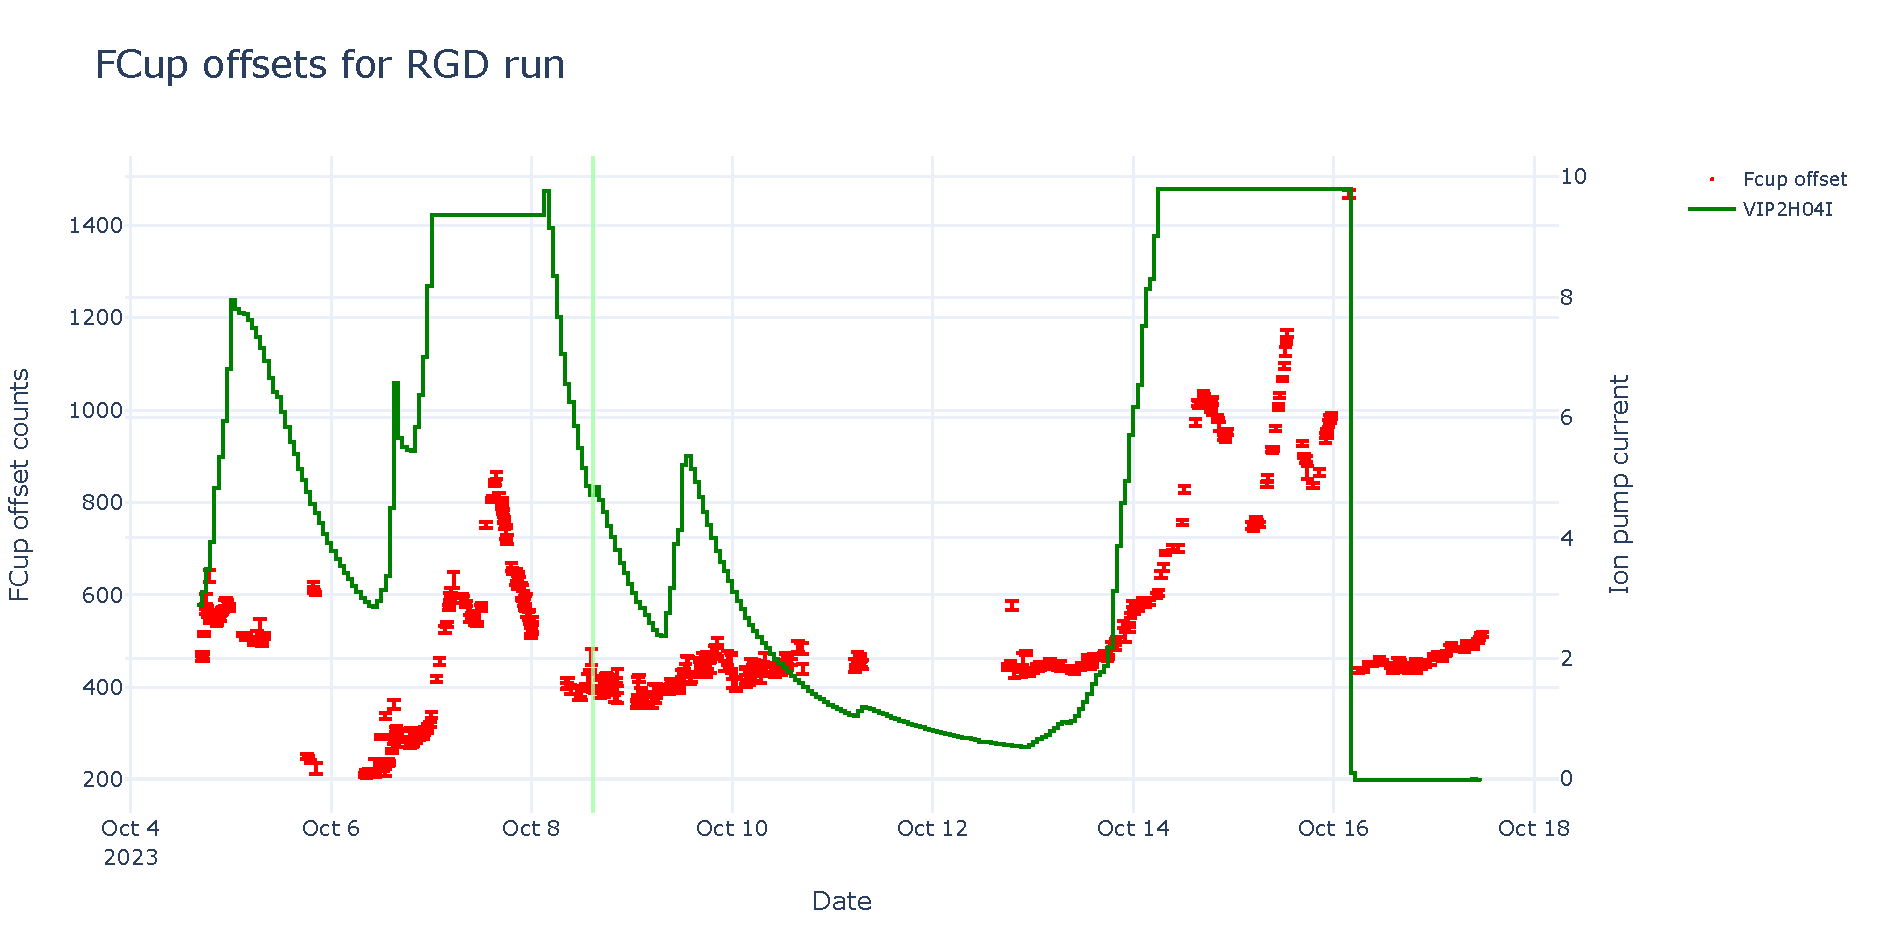
\includegraphics[width=0.95\textwidth]{figures/FCup_offsets_early_part_RGD.pdf}
\caption{Recomputed FCup offsets $R_0$ (red, left axis) and the ion pump current \code{VIP2H04I}
(green, right axis) for the first two weeks of RGD. The thin green band on October 8 marks the
BPM calibration current scan (Sect.~\ref{sec:bpmcal}), when the offset was stable at
$\approx 400$\,Hz.}
\label{fig:offset_early}
\end{figure}

\begin{figure}[H]
\centering
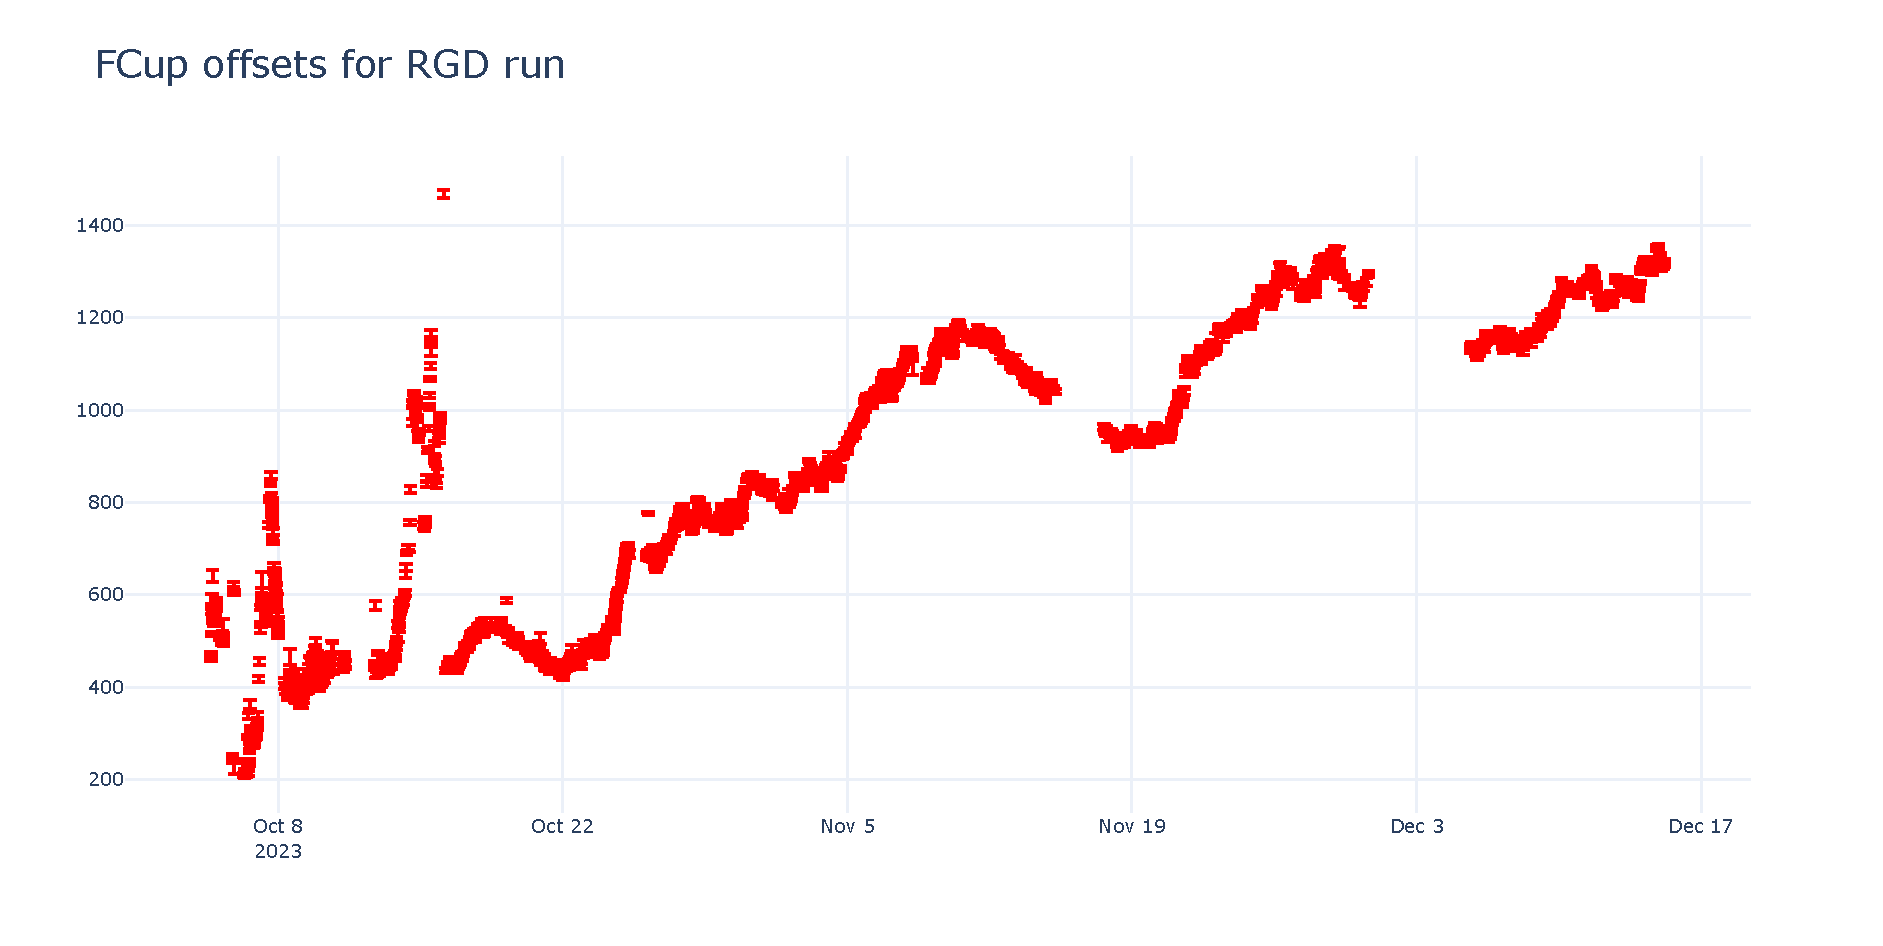
\includegraphics[width=0.95\textwidth]{figures/FCup_offsets_all_data_RGD.pdf}
\caption{Recomputed FCup offset (scaler counts at zero beam) for the full RGD run period.}
\label{fig:offset_all}
\end{figure}

%======================================================================
\section{Recomputing the FCup offset}
\label{sec:offset}
%======================================================================
Since the online offset is unreliable, $R_0$ was recomputed from the data itself, using every
beam trip as a zero-current measurement (\code{RGD\_Get\_Current\_Data.py}):
\begin{enumerate}
  \item Beam trips are found in \IC\ as a sample with $I < \SI{0.01}{\nano\ampere}$ whose preceding
        sample was at least \SI{0.2}{\nano\ampere} higher. Because MYA only stores changed values, the next
        \IC\ sample marks the beam restore.
  \item All \code{scalerS2b} samples between the trip and \SI{2.5}{\second} before the restore are
        selected. The \SI{2.5}{\second} margin absorbs timing differences between the BPM and scaler
        readouts.
  \item The trip is accepted if it contains more than 30 scaler samples ($\gtrsim$30\,s) and the
        sample standard deviation is below 20\,Hz. The mean of the samples is $R_0$ at that time.
  \item Each \code{scalerS2b} sample is assigned the most recent preceding $R_0$ (forward fill);
        samples before the first trip get the first $R_0$.
\end{enumerate}
Fig.~\ref{fig:offset_example} illustrates the method for one day. During the calibration scan of
October 8, the FCup current computed from \code{scalerS2b} with the recomputed offset agrees with
the online \code{scaler\_calc1b} to better than 0.03\% in slope (fit slope $0.99979\pm0.00012$),
which validates the method and confirms that the online offset was correct at that time.

\begin{figure}[H]
\centering
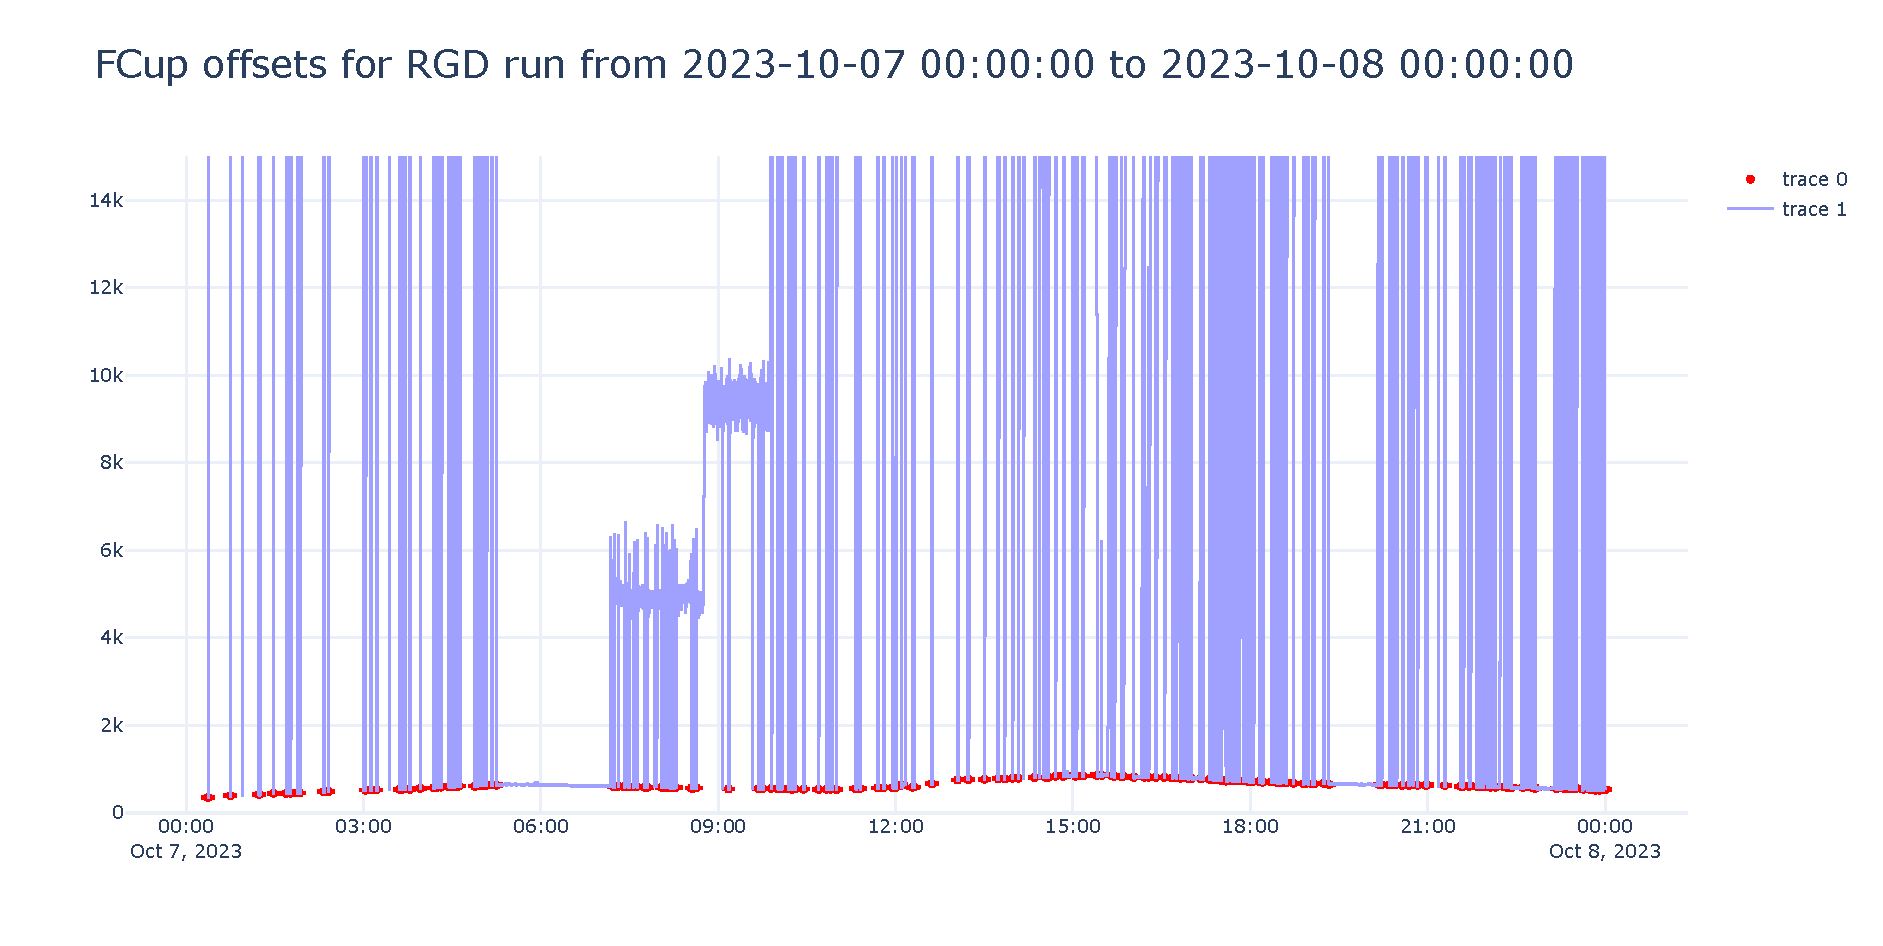
\includegraphics[width=0.95\textwidth]{figures/Compute_FCup_offsets_example.pdf}
\caption{Raw FCup scaler \code{scalerS2b} (blue) on October 7, 2023, and the offsets computed
from the beam trips (red points with standard deviation as error bars).}
\label{fig:offset_example}
\end{figure}

%======================================================================
\section{BPM calibration against the FCup}
\label{sec:bpmcal}
%======================================================================
\subsection{Calibration data}
On October 8, 2023, R.~Paremuzyan performed a current scan for the beam blocker calibration
(logbook entries
\href{https://logbooks.jlab.org/entry/4195353}{4195353},
\href{https://logbooks.jlab.org/entry/4195624}{4195624},
\href{https://logbooks.jlab.org/entry/4195622}{4195622},
\href{https://logbooks.jlab.org/entry/4201989}{4201989}).
Two current ramps of 5 to \SI{200}{\nano\ampere} were taken with the beam blocker out
(Fig.~\ref{fig:ramp}): 14:17:26--14:30:24 (interpreted as the empty target) and 14:34:16--14:49:12
(CuSn target). The logbook does not state which ramp corresponds to which target.
This scan is the best available calibration: the FCup offset was stable, no blocker attenuation
applies, and it spans the full range of currents used in the experiment.

\begin{figure}[H]
\centering
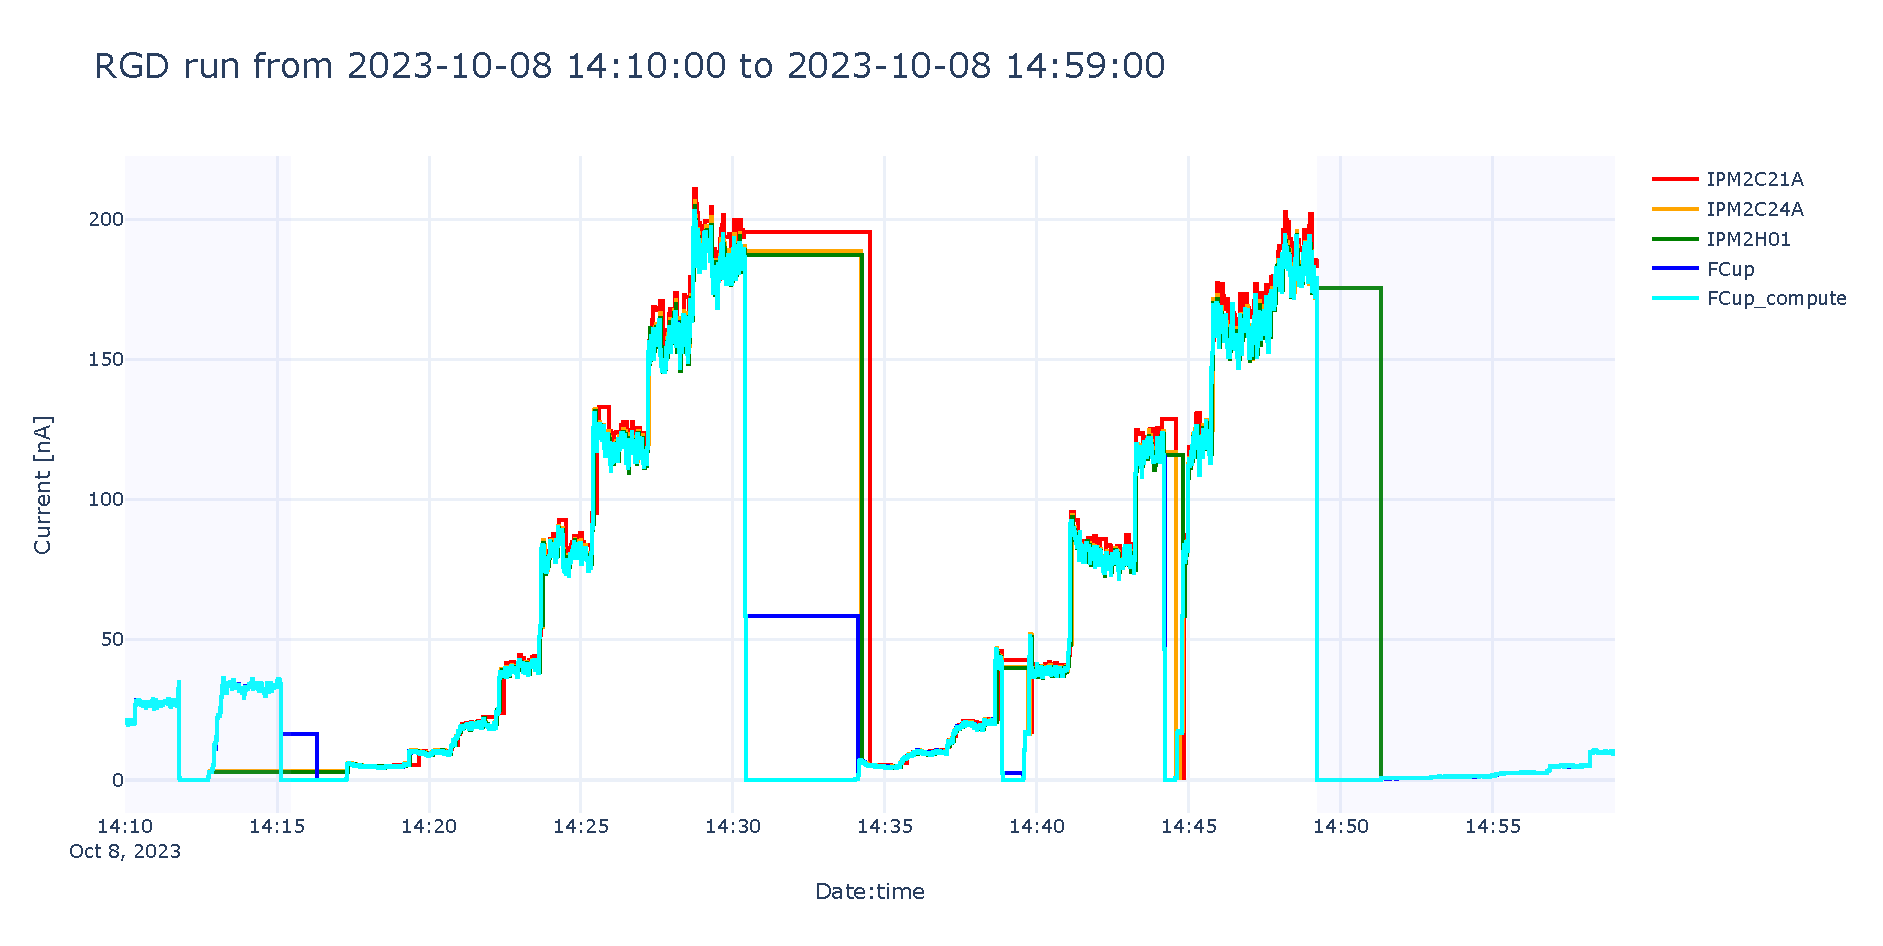
\includegraphics[width=0.95\textwidth]{figures/RGD_oct_8_current_ramp.pdf}
\caption{Currents during the October 8 current scan. Only samples where the BPM agrees with the
FCup to within 5\% are drawn. The shaded regions at the edges are periods with the beam blocker in.}
\label{fig:ramp}
\end{figure}

\subsection{Fit}
For each BPM the samples are paired with the FCup sample (\code{scaler\_calc1b}) at the same time
(forward-filled). Pairs that differ by more than 25\% are dropped, which removes the transition
regions at beam trips and current steps. A straight line
\begin{equation}
  I_\mathrm{FC} = a\, I_\mathrm{BPM} + b
  \label{eq:cal}
\end{equation}
is fit with orthogonal distance regression (\code{scipy.odr}), which accounts for the fluctuations
in both quantities (Fig.~\ref{fig:fit}). The results are listed in Table~\ref{tab:cal}. The empty-target
ramp is used for the final calibration; the other determinations serve as cross-checks.
The slopes agree at the 0.3--0.6\% level. The offsets $b$ are consistent with zero
within their uncertainties of $\approx \SI{0.16}{\nano\ampere}$.

\begin{figure}[H]
\centering
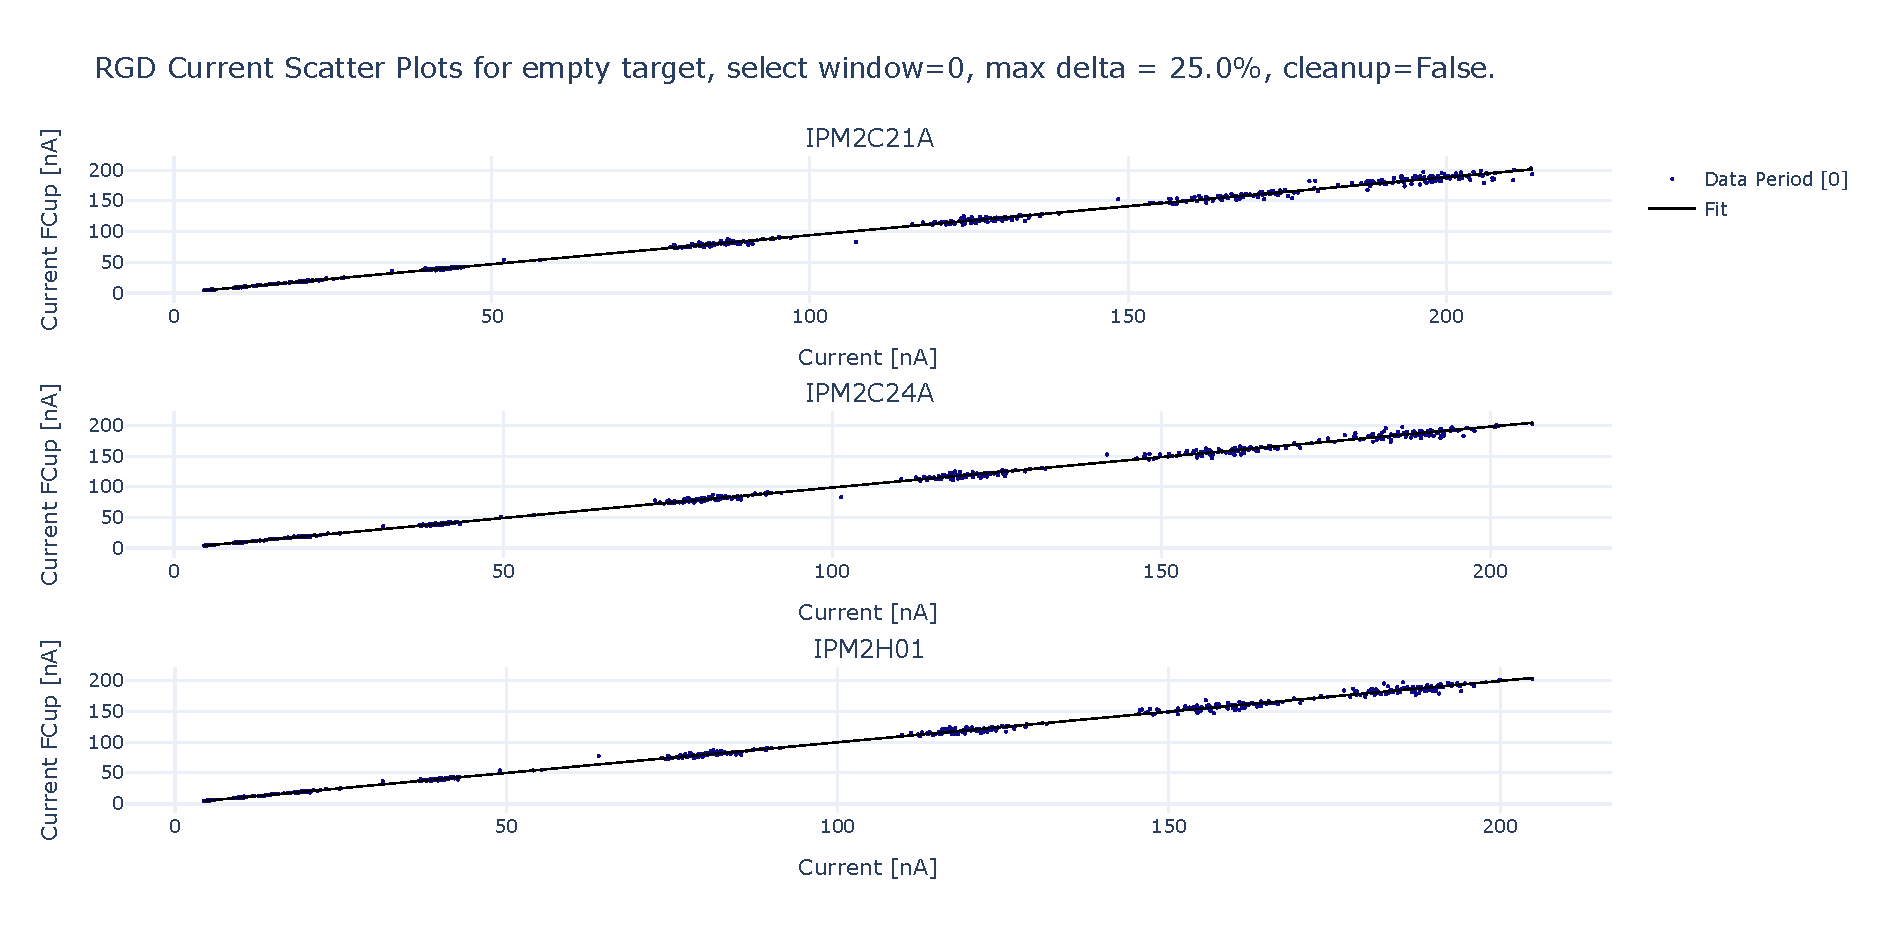
\includegraphics[width=0.95\textwidth]{figures/RGD_empty_target_fit.pdf}
\caption{FCup current versus BPM current for the empty-target ramp, with the linear ODR fit.}
\label{fig:fit}
\end{figure}

\begin{table}[H]
\centering
\caption{Calibration constants of Eq.~(\ref{eq:cal}). The LD2 values come from the October 6
luminosity scan (LD2 target, runs 18318--18325). The ``Online'' values are those posted in logbook entry
4201989, inverted to the form of Eq.~(\ref{eq:cal}).}
\label{tab:cal}
\begin{tabular}{lcccc}
\toprule
 & \multicolumn{2}{c}{\textbf{Empty target (used)}} & CuSn & LD2 lumi scan \\
BPM & $a$ & $b$ [nA] & $a$ & $a$ \\
\midrule
\IC & $0.94360\pm0.00148$ & $-0.194\pm0.167$ & $0.94710$ & $0.94364$ \\
\ID & $0.99133\pm0.00144$ & $-0.182\pm0.154$ & $0.99548$ & $0.99407$ \\
\IH & $0.99848\pm0.00144$ & $-0.011\pm0.153$ & $1.00466$ & $1.00343$ \\
\midrule
\multicolumn{5}{l}{Online (empty): \IC\ $a=0.9497$, $b=-0.302$; \quad \ID\ $a=0.9982$, $b=-0.211$} \\
\bottomrule
\end{tabular}
\end{table}

The calibration is applied sample by sample to the full BPM time series,
$I^\mathrm{corr}_\mathrm{BPM}(t) = a\, I_\mathrm{BPM}(t) + b$, and stored as column \code{corr}
in \code{RGD\_mya\_data\_corr.h5}.

\subsection{BPM behavior at beam trips}
After a beam trip the BPMs respond later than the FCup and then overshoot for several seconds
(Fig.~\ref{fig:details}). Integrated over the recovery window of $\sim$7\,s this mostly
cancels, and the effect on a run-integrated charge is negligible. These regions are excluded from
the fits via the 25\% agreement requirement but are \emph{not} removed when integrating the charge.

\begin{figure}[H]
\centering
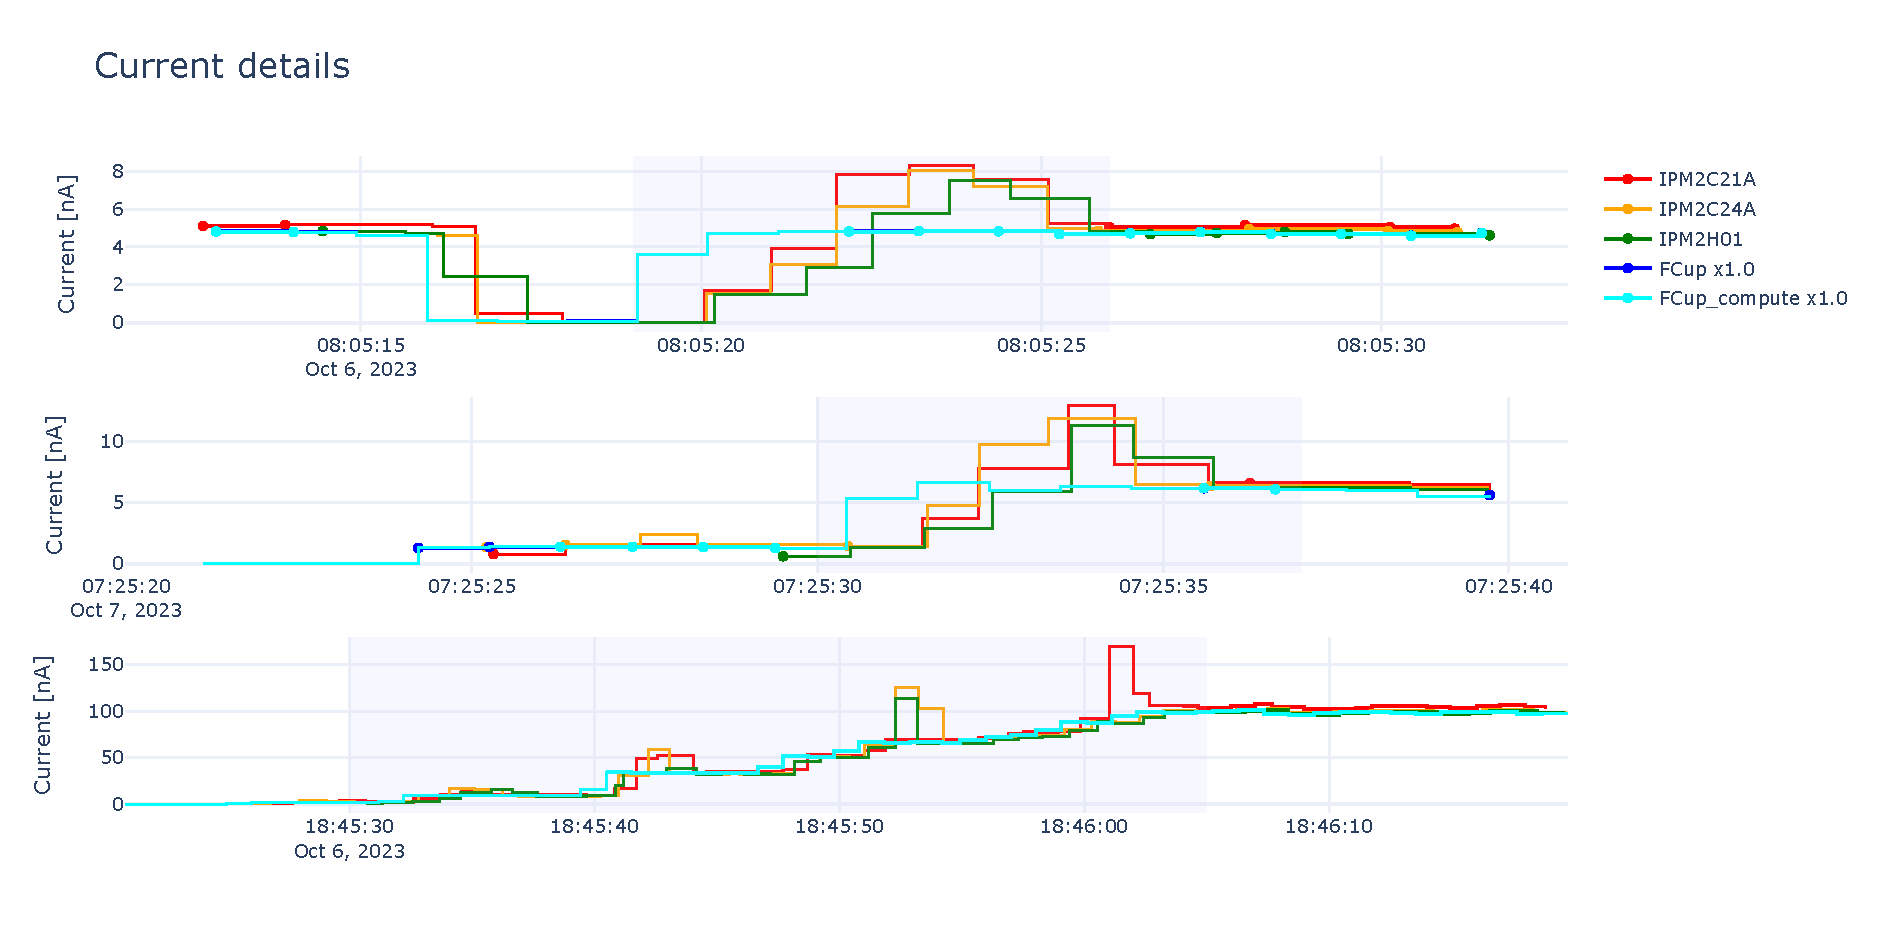
\includegraphics[width=0.95\textwidth]{figures/RGD_current_details.pdf}
\caption{Beam restores after a trip at \SI{5}{\nano\ampere} (top, middle) and with a slow ramp to
\SI{100}{\nano\ampere} (bottom). The FCup (blue, cyan) recovers first; the BPMs lag and overshoot.
The shaded regions show the recovery window.}
\label{fig:details}
\end{figure}

%======================================================================
\section{Charge per run}
\label{sec:charge}
%======================================================================
\subsection{Integration}
For each run $r$ with start and end times from the RCDB, and each BPM $k$, the live-time weighted
charge is
\begin{equation}
  Q_k^{(r)} = \int_{t_\mathrm{start}}^{t_\mathrm{end}} I^\mathrm{corr}_{k}(t)\,
              \frac{L_\mathrm{DAQ}(t)}{100}\, dt ,
  \label{eq:charge}
\end{equation}
where $L_\mathrm{DAQ}$ is \code{B\_DAQ:livetime} in percent. The live time is evaluated at each
BPM sample time by forward fill, and the integral is done with the trapezoidal rule over the
BPM samples (with $I$ in nA and $t$ in ms, a factor $10^{-9}$ gives mC). Of the available
live-time channels, only \code{B\_DAQ:livetime} was found to be consistently reliable.
Samples with invalid (\code{NaN}) values are removed.

As a cross-check, the calibration was also applied to the already-integrated live-time corrected
charge, $Q \approx a\,Q^\mathrm{LT} + b\,\Delta t$, with $\Delta t$ the run duration
(\code{\_corr2} columns). This differs from Eq.~(\ref{eq:charge}) only because $L_\mathrm{DAQ}$
is not constant during a run. For runs with $\geq 20$M events the median difference is 0.17\%,
and the summed charges agree to 0.05\%.

\subsection{Final charge and uncertainty}
The charge for each run is the mean of the three BPMs, and its uncertainty the standard deviation:
\begin{equation}
  Q^{(r)} = \frac{1}{N}\sum_{k} Q_k^{(r)}, \qquad
  \sigma_Q^{(r)} = \sqrt{\frac{1}{N}\sum_{k}\left(Q_k^{(r)} - Q^{(r)}\right)^2 }.
\end{equation}
Normally $N=3$. For runs where \IH\ was not working (raw charge $< \SI{0.001}{\milli\coulomb}$),
\IH\ is dropped and $N=2$. All three BPMs are treated equally. Two of them (\ID\ and \IH) agree
more closely with each other, but there is no way to show that the third one is the one that drifts.

Fig.~\ref{fig:lt} shows the per-run charges after live-time correction only. The uncalibrated BPMs
disagree by up to 4\%, and the disagreement is remarkably constant over the run. After calibration
(Fig.~\ref{fig:full}) the three BPMs agree to within $\pm 0.5\%$. The remaining spread is not
constant in time, see for example the jump of \IC\ around November 1. This indicates slow drifts
of the BPM gains, which cannot be corrected without a working FCup. The distribution of the
deviations is shown in Fig.~\ref{fig:diffs}.

\begin{figure}[H]
\centering
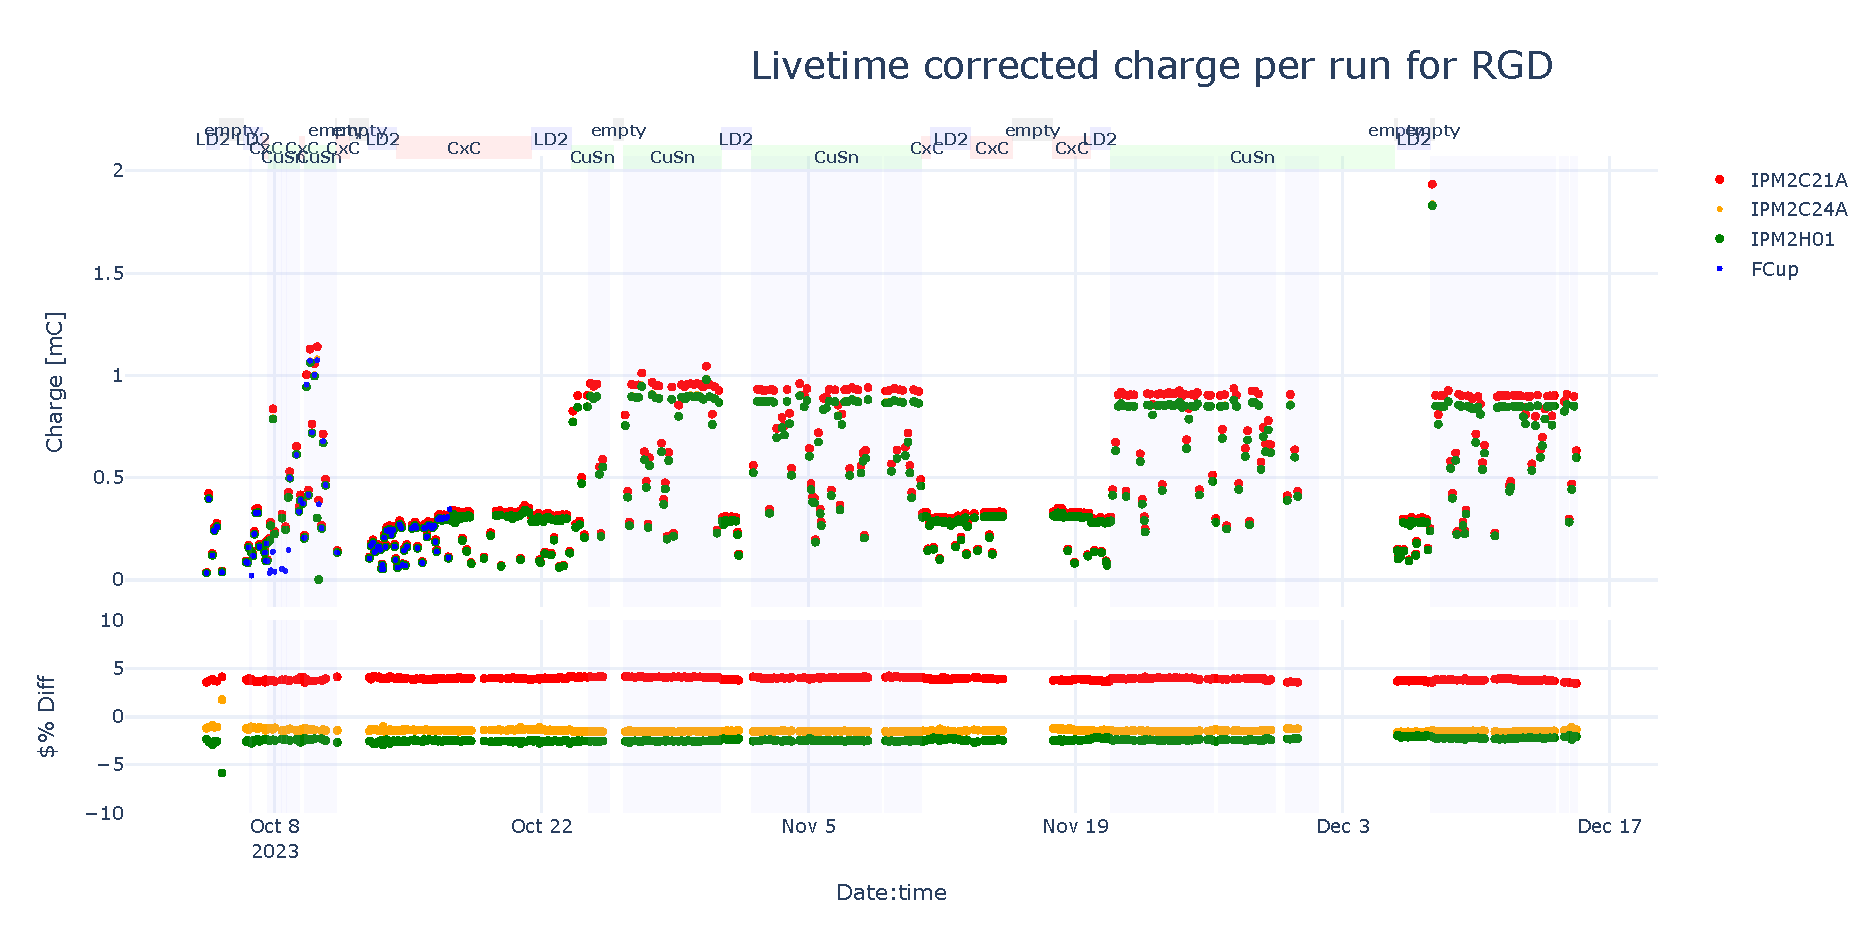
\includegraphics[width=0.95\textwidth]{figures/RGD_LT_corrected_charge_per_run.pdf}
\caption{Live-time corrected charge per run (runs with $\geq 20$M events) \emph{before} the BPM
calibration. The bottom panel shows the percent deviation of each BPM from the three-BPM mean.
The FCup is shown only before 2023-10-17. The target in use is labeled at the top; shaded regions
indicate the beam blocker was in.}
\label{fig:lt}
\end{figure}

\begin{figure}[H]
\centering
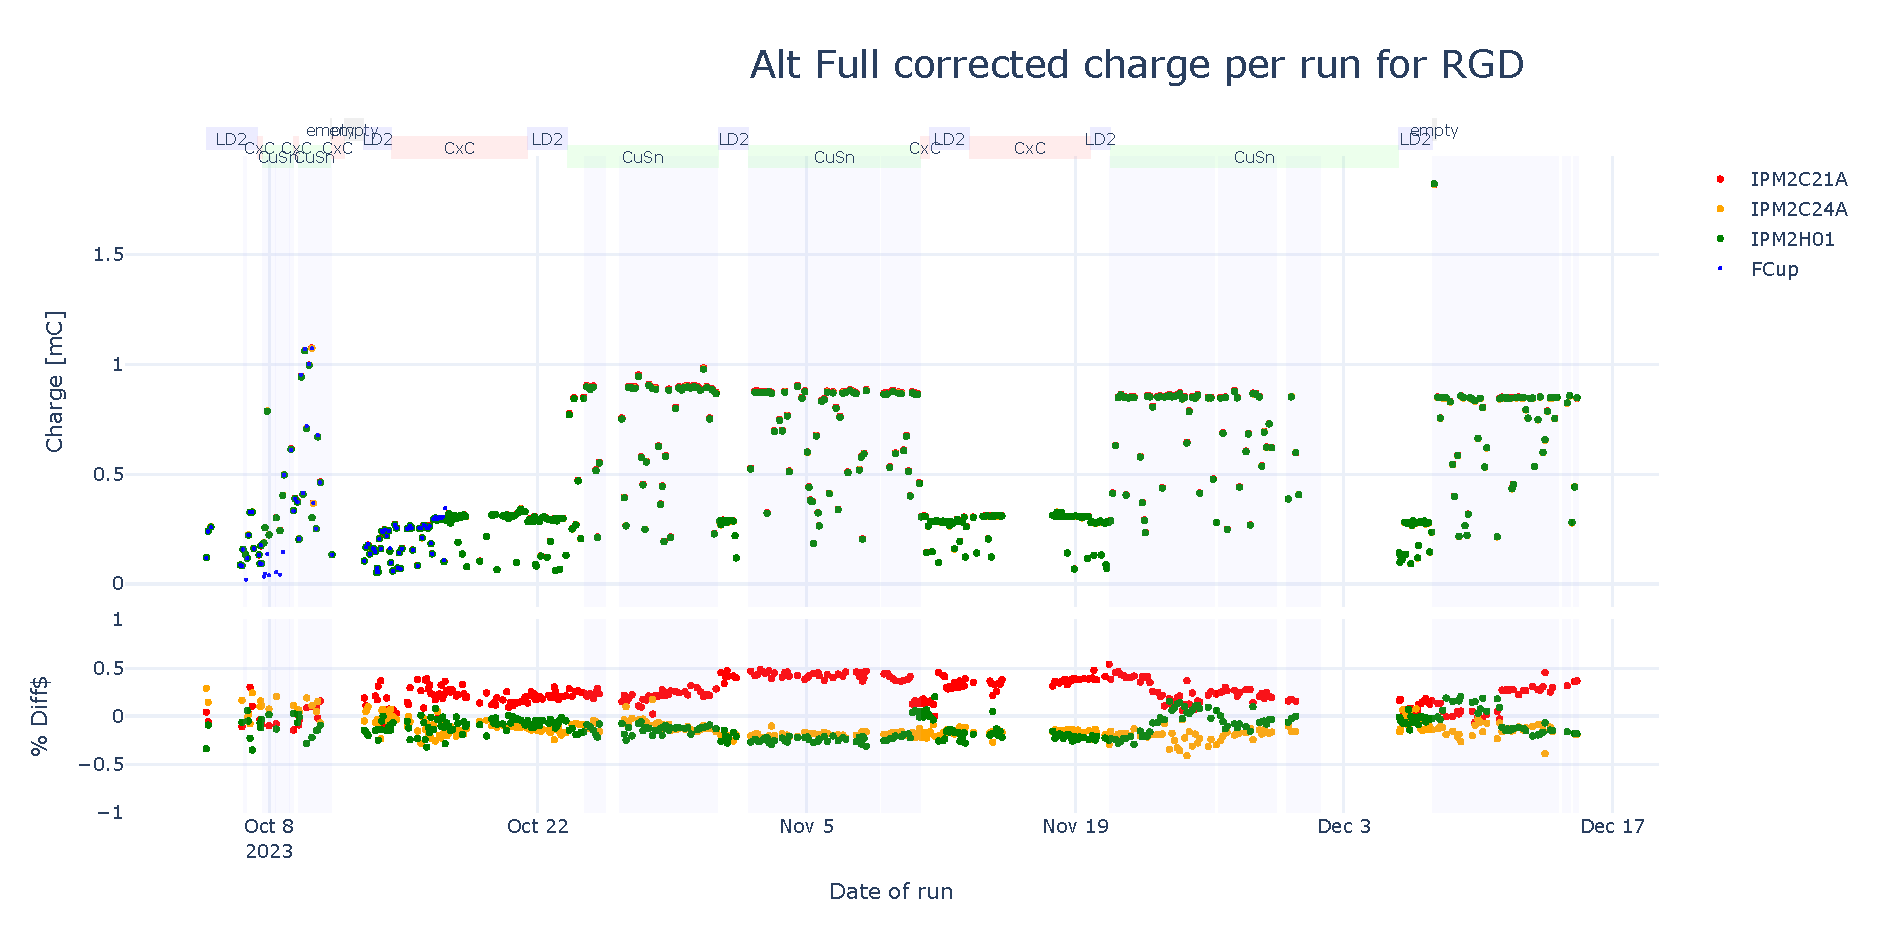
\includegraphics[width=0.95\textwidth]{figures/RGD_Full_corrected_charge_per_run2.pdf}
\caption{Final, fully corrected charge per run, Eq.~(\ref{eq:charge}), for runs with $\geq 20$M
events. Bottom: percent deviation of each calibrated BPM from the mean (note the
$\pm 1\%$ scale, compared with $\pm 10\%$ in Fig.~\ref{fig:lt}).}
\label{fig:full}
\end{figure}

\begin{figure}[H]
\centering
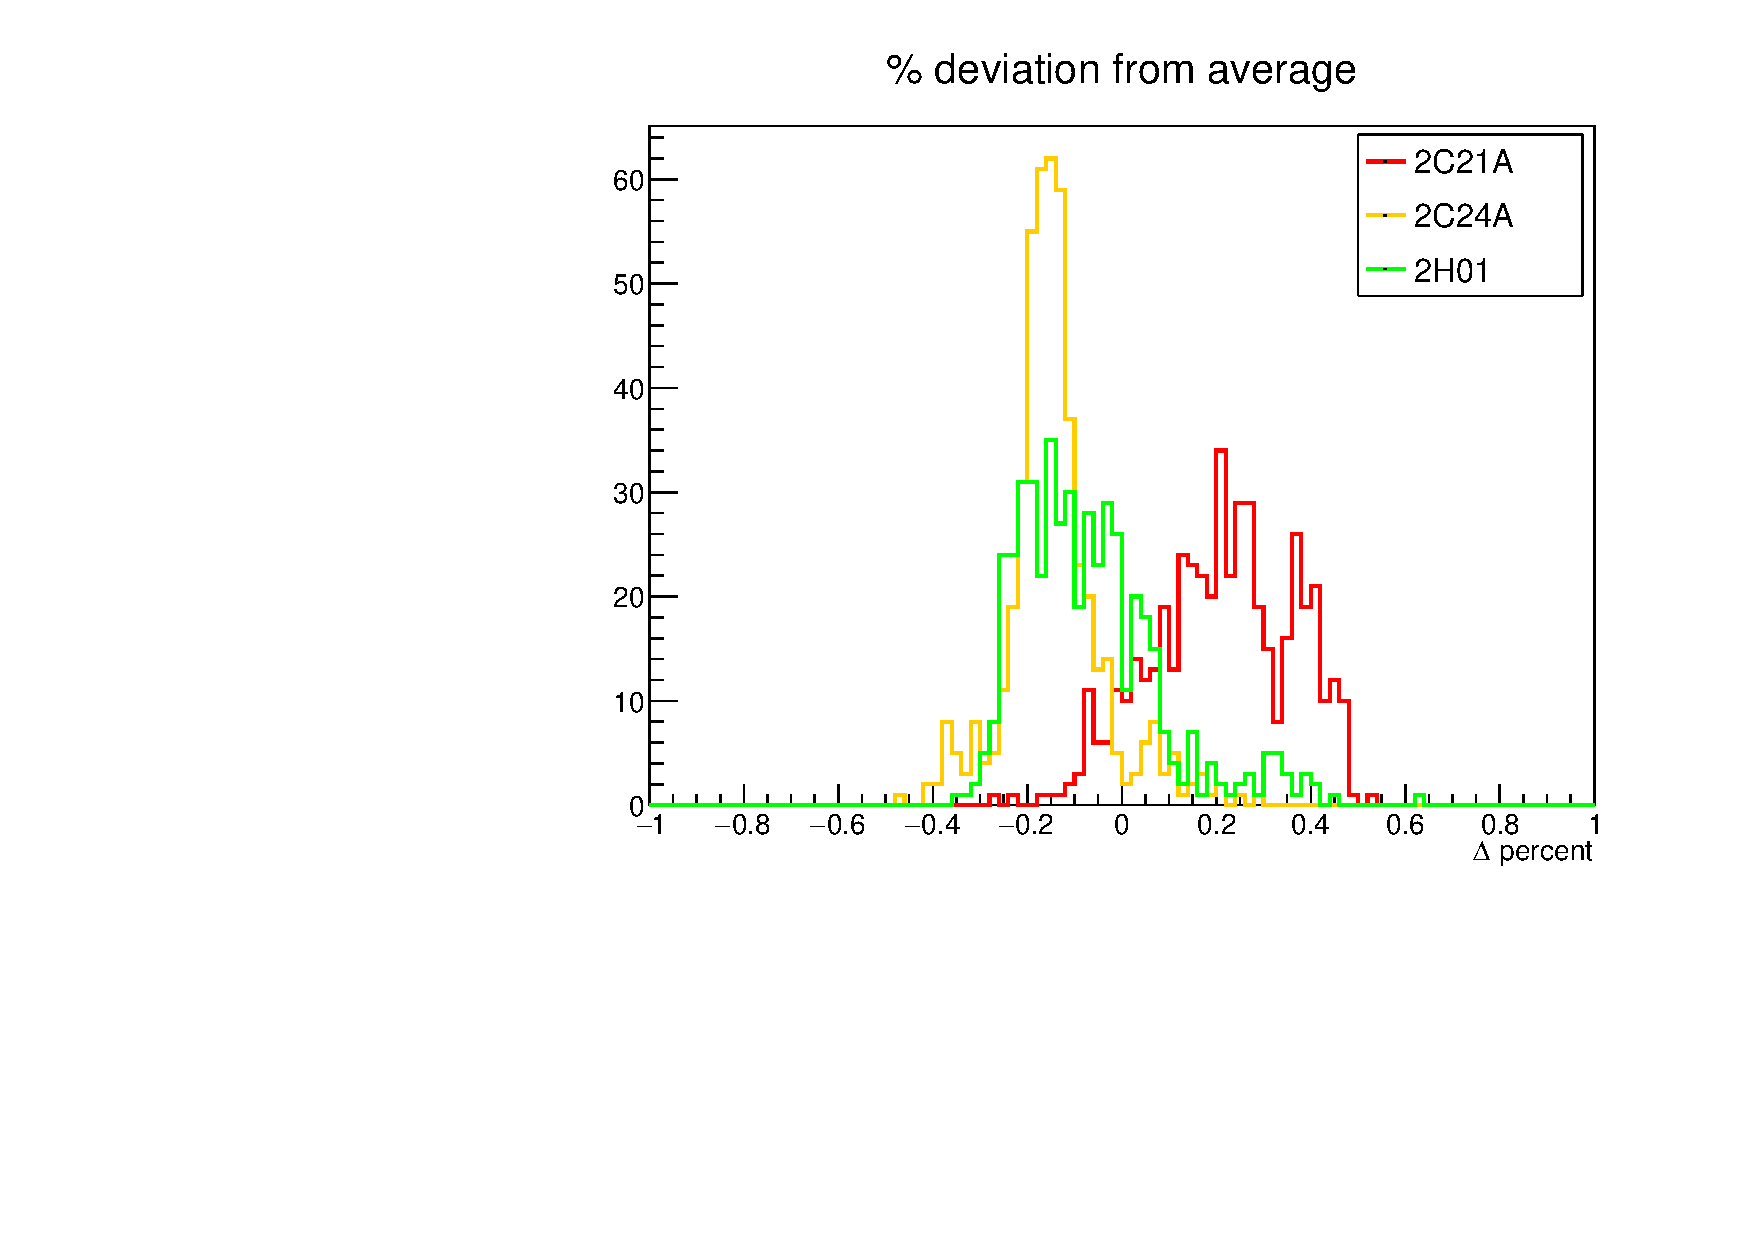
\includegraphics[width=0.6\textwidth]{figures/RGD_Full_corrected_charge_per_run2_diffs.pdf}
\caption{Distribution of the percent deviation of each calibrated BPM from the three-BPM mean,
for runs with $\geq 20$M events.}
\label{fig:diffs}
\end{figure}

\subsection{Results}
\begin{table}[H]
\centering
\caption{Accumulated charge per target, all 662 runs.}
\label{tab:result}
\begin{tabular}{lrr}
\toprule
Target & Runs & Charge [mC] \\
\midrule
LD2   & 165 & 30.69 \\
CxC   & 137 & 27.72 \\
CuSn  & 349 & 170.79 \\
Empty &  11 & 2.16 \\
\midrule
Total & 662 & 231.36 \\
\bottomrule
\end{tabular}
\end{table}

For runs with at least 20M events, the median relative uncertainty $\sigma_Q/Q$ is 0.18\%, and the
charge-weighted average is 0.36\%. This uncertainty only reflects the relative disagreement
between the BPMs. It does not include the uncertainty of the absolute FCup calibration
or common-mode drifts of all three BPMs after October 8. A conservative estimate of the latter
is the 0.3--0.6\% spread between the calibration slopes obtained with different targets and dates
(Table~\ref{tab:cal}).

\subsection{Known limitations}
\begin{itemize}
  \item The calibration offset $b$ is applied to all samples, including those during beam trips
        where the true current is zero. With $|b|\lesssim\SI{0.2}{\nano\ampere}$ this is a
        negligible bias ($<0.1\%$ for typical currents and downtimes), and $b$ is consistent with zero.
  \item The calibration is taken from a single 13-minute scan on October 8. Long-term BPM drift
        can only be bounded by the inter-BPM spread.
  \item The target in use is taken from the RCDB. It is only defined during runs.
\end{itemize}

%======================================================================
\section{Output files}
%======================================================================
\begin{itemize}
  \item \code{RGD\_charge\_final.txt}, \code{RGD\_charge\_final.csv}: run number, charge [mC], uncertainty [mC].
  \item \code{RGD\_charge\_final.xlsx}: as above plus the three calibrated BPM charges.
  \item \code{RGD\_all\_runs\_fully\_corrected.xlsx}: run information from the RCDB with raw and corrected charges.
  \item \code{RGD\_all\_runs\_fully\_corrected\_all\_corrections.xlsx}: all intermediate correction columns.
\end{itemize}

\end{document}
